%!TEX root = ../main.tex
\chapter{Reverse Engineering Methods, Tools, and examples}
Because reverse engineering serves a wide variety of purposes, there is an equally broad range of methods and strategies employed to achieve those goals. In \textit{Reversing: Secrets of Reverse Engineering}, these methods are generally categorized into two primary types. The first type focuses on large-scale observation of a program and is referred to as system-level reversing \cite{Reversing}. System-level reversing seeks to determine the overarching structure of a program and identify potential areas of interest within it. Once a general understanding of the program’s layout has been established, the analysis can proceed to the second type: code-level reversing. Code-level reversing delves deeper into the specifics of a program’s inner workings, offering detailed insights into particular segments of code and uncovering how algorithms and functionalities are implemented.

System-level reversing is achieved by running an array of specialized tools on a program and observing the services provided by the operating system. These observations gather information on how the program interacts with system resources, tracks input and output operations, and reveals characteristics of the program’s executable files. Much of this data is supplied by the operating system, as any portion of a program that interacts with components outside itself must necessarily communicate through the OS. As a result, effective system-level reversing demands a strong familiarity with the operating system’s internal workings, making it invaluable for reverse engineers to develop deep expertise in the OS environment they are targeting.

Code-level reversing, by contrast, is a far more complex and meticulous process. It involves extracting algorithms, logic, and design concepts directly from a program’s binary code. This task requires a robust background in reverse engineering techniques, software development practices, CPU architecture, and operating system internals. Even when working with readable, well-documented source code, modern software systems can be enormously complex. For instance, the program examined in this project comprises 21 frameworks, contributions from at least three separate companies, and potentially tens or even hundreds of thousands of lines of code. Moreover, when high-level code is compiled into binary instructions, a single line of code can transform into ten or more lines of low-level machine instructions. Reversing production-level software from binary back to source code is thus an almost incomprehensibly difficult endeavor. Thankfully, multiple methodologies and a variety of specialized tools have been developed to aid in effective code-level reversing, making this seemingly impossible task more approachable for skilled practitioners.

\subsection{Static Analysis}

Static analysis is the practice of analyzing code without executing it. This approach allows reverse engineers to study the structural and logical components of a program in a controlled environment, free from the risks associated with running potentially malicious code. Static analysis can also serve as a valuable precursor to dynamic analysis, helping to identify key areas of interest for more in-depth examination later.

Static analysis tools operate at both the source code level, when code has not yet been compiled, and at the machine language level, analyzing binary or assembly-level code. Reverse engineers frequently use static analysis tools to disassemble machine code into assembly instructions, enabling them to examine and interpret how different sections of code relate to one another. While retrieving disassembled code is one of the most fundamental functions of static analysis tools, many modern tools offer a host of additional features, such as graphical representations of control flow, cross-referencing functions, and identifying potential vulnerabilities. These tools are often designed to provide reverse engineers with a starting point, helping them navigate the often bewildering world of assembly-level functions and binary logic.

\subsubsection{Disassembler}
One of the most key static analysis tools for a reverse engineer is a disassembler. 
Disassemblers are applications that take in a program’s executable file and generate a file with the assembly code.
This isn’t too difficult because assembly is just a text translation of the machine readable binary code. 
Unfortunately, that makes it a lot less clear than higher level programming languages.  
Disassembly is also unique to a person’s processor, but there are disassemblers that can support more than one CPU architecture.
Some examples of disassemblers are IDA, Binary Ninja, Hopper, Ollydbug, Radare2, and Ghidra.

\subsubsection{Decompiler}
Decompilers are similar but more complex than disassemblers.
Instead of just producing the assembly language code, decompilers attempt to produce high-level readable code. 
They attempt to produce something that looks as close to the source code as possible by reversing the compilation process~\cite{Reversing}.
The front end of the decompiler decodes low-level assembly instructions and translates it into an intermediate representation specific to the decompiler. 
The intermediate representation is then iterated on to remove as many extraneous details as possible while preserving the important details. 
Lastly the back end takes the polished up intermediate representation and translates it again into a high level language.

While this may sound like a simple way to retrieve the source code, it is highly unlikely the high level language returned will be something that actually matches. 
Anyone who has ever run text through a translation website multiple times knows that each iteration causes a loss in fidelity and oftentimes the end result will be gibberish. 
Decompilers go a step further and have no immediate knowledge of things like function or variable names and structures. 
This does not make them useless, though. For example, a text translator will usually return your original result when given a simple phrase. 
Similarly a decompiler will most likely be able to pick up on more straightforward functions such as adding a + b. 
Decompilers offer hints and snippets into what the source code may look like which is valuable information for a reverse engineer. 
Most of the examples for disassemblers listed also count as decompilers.

\subsubsection{Dumping Tools}
Executable dumping is usually the first step in reverse engineering a program. 
Executable dumping helps inform a reverse engineer what a program does, how it interacts with external elements, and general knowledge of how a file is structured. 
Using dumping tools, a reverse engineer will start by figuring out what type of file they’re dealing with. 
They will then start to unpack the format. 
Extracting strings will immediately offer insight into what language the source code is written in, what library modules it uses, what kinds of data it is dealing with, and what the goals of program functions may be. 
Other useful information we can retrieve is the layout of the file in memory and what the general logical structure of the file is. Once we know the type of file we also know which tools we can use. 
For example, some debuggers only work with certain high and low level languages. 
Some popular executable dumping programs are ones already built into your machine like DUMPBIN for Windows or otool for Mac. 

Otool is identifies a file's Mach header. 
On systems with a Mach kernel like macOS and iOS, the executable binaries they use will have a Mach header. 
All headers have a magic number to identify them. Thin binaries only have that number while fat binaries with fat headers will have locations of the other executable's headers in them.

\subsection{Dynamic Analysis}

Dynamic analysis occurs when a program—or specific sections of it—is executed during the analysis process. This approach provides unique insights into how software behaves in real time, revealing execution paths, input/output relationships, and interactions with external systems. Because running an unknown program can produce unpredictable and potentially harmful results, it is safest to conduct dynamic analysis within a secure, isolated, or sandboxed environment. Virtual machines are commonly used for this purpose, as they are easy to set up, control, and reset between tests.

A wide variety of tools contribute to dynamic analysis. Any tool that executes code and monitors its behavior falls under this category. Some dynamic analysis tools run entire programs to observe overall functionality, while others focus on specific sections, functions, or even single instructions. Additionally, tools that monitor a program’s external environment during execution—for example, capturing network traffic, tracking file system changes, or observing registry modifications—are also considered part of dynamic analysis. Together, these tools give reverse engineers a powerful way to understand not just how a program is built, but how it behaves in practice.

\subsubsection{Debugger}
Debuggers are a tool usually used for developers to locate and work through errors in their programs, but they’re also vital tools in reverse engineering. 
Many debuggers can work through assembly language. 
While assembly language may be difficult for a human to parse through, it is the exact same logic that gets broken down and sent to a computer meaning that the computer can show what each assembly instruction is intended to do. 
Most debuggers software engineers use were actually designed from the ground up with the purpose of stepping through assembly code. 
The debugger can show the state of CPU registers along with a memory dump that shows what’s in the stack. 
Debuggers usually contain disassemblers which as discussed is a vital reverse engineering tool. 
Many debuggers also contain both software and hardware breakpoints. 
Software breakpoints are instructions added into the code during runtime to pause and hand control over to the debugger. 
Hardware breakpoints are a CPU feature which allow the processor to pause execution when a certain memory address is reached and hand control over to the debugger. 
A reverse engineer can use insert breakpoints at data structures of interest and use the debugger to reveal what they are. 
Debuggers also offer a clear view of registers and memory to aid in a reverse engineer's ability to process low level information.

\paragraph{\underline{User Mode Debuggers}}
Most debuggers that a programmer will use are user mode debuggers.
They run on a system like any other application then seize control of the target program to debug ~\cite{Reversing}.
An advantage to them is that they are easier to set up and navigate than their kernel-mode counterparts.
Usually it’s fine to stay limited to user mode viewing of an application. 
It only creates troublesome limitations when the target application has kernel mode components such as device drivers. 
User mode debuggers are also not always sufficient when trying to debug a program before it reaches the main entry point. 
These kinds of programs are usually ones that have a lot of statically linked libraries in the executable. 
The final and most likely to be problematic issue is that user-mode debuggers can only view a single process in a program. 
This can cause issues when the target application has processes that interact in unknown ways. 
The user may not know which process to zero in on that has the code of interest.

\paragraph{\underline{Kernel Mode Debuggers}}
Kernel mode debuggers are different from user-mode debuggers because they capture the entire system and not just a single process. 
Instead of running atop the operating system, kernel mode debuggers sit alongside the system kernel and stay ready to capture the entire system’s stats. 
Kernel mode debuggers can be more helpful to reverse engineers because they offer more clues as to what’s going on with the system. 
A key tool for kernel-mode debuggers is that they allow the placement of low level code breakpoints. 
As a reverse engineer working with assembly code, being able to test different sets of assembly instructions that may be the code section a reverser is looking for is incredibly useful.

For example, picture a scenario where a reverse engineer is looking for the API responsible for handling moving windows? 
That will need to be managed by a windows manager in the kernel. 
The complexity is introduced when trying to identify which API moves a particular window. 
Since there are multiple APIs that can be used to move a window, pinpointing the one you are trying to focus on is a difficult task. 
This is where kernel mode debuggers come in handy. 
Low level breakpoints in the operating system responsible for shifting windows around will help you identify which API is getting called when a window is moved~\cite{Reversing}. 
From there the reverse engineer will be able to hone in on that API.

Unfortunately, kernel mode debuggers come with their own drawbacks. 
Setting them up can be challenging because they require access to the full system. 
They need to suspend the entire system while running so they can go line by line, which means the system can no longer have multiple threads going~\cite{Reversing}. 
They will also usually need to be set up inside a virtual machine which will be discussed in a later section~\cite{PracticalRE}. 
These are reasons why a reverser should exhaust their other options before jumping into using a kernel mode debugger. 
Still, they are powerful tools when the scenario calls for it.

\subsubsection{System Monitor}
System monitoring can be a crucial part of the reverse engineering process. 
In some cases, a reverse engineer can figure out what they need through system monitoring tools without ever looking at the decompiled code. 
System monitoring tools can capture what happens between the code and hardware using the intermediate channels of input/output~\cite{Reversing}. 
For local system monitoring, tools monitor things such as file operations (creating, deleting, moving, etc). 
For programs that communicate over networks, system monitoring might look like recording all TCP/UDP network traffic. 
System monitoring tools are commonly used in virtual machines.


\subsubsection{Virtual Machine}
Many programmers will encounter virtual machines (VM) at some point during their career. 
It’s not uncommon for an application to interface exclusively with one type of operating system. 
One reason is because writing applications to work with different operating systems adds time and complexity that not all programmers can afford.
Choosing to write in a high level language may make code more portable because there’s more verbose built-in libraries or interpreters that deal with the specifics of the systems without the need for any programmer intervention.
But high level languages often trade performance for convenience which is not a trade that a developer working with large amounts of data can necessarily afford to take.
What happens when a developer has an application that runs on Windows while they have a Mac? 
This is where a virtual machine enters into the mix. Virtual machines are safe sandboxed environments that work as miniature computers with their own operating systems within a computer. 
They are constructed with an interpreter and bytecode. 
During compile time, select code snippets are compiled specific for the VM target architecture and then inserted into the program along with the interpreter. 
During run-time, the interpreter begins executing the bytecode. 
Virtual machines are costly to implement because they are so expansive which is why only the necessary code snippets get rendered~\cite{MasteringRE}.
Because virtual machines work in their own isolated environment, they offer powerful protections against unknown or potentially malicious software. 
This makes them a useful tool for reverse engineers who deal with software that they do not know the contents of. 
The level of control over virtual machines also makes them a useful tool because there is ultimate knowledge of system conditions.


\section{Protocol Analysis}

Communication protocols form the essential foundation for structured exchanges of information between different systems and components. Many applications, especially those that involve interoperability between different platforms or devices, depend on well-defined formats for sending and receiving messages. However, in cases where official protocol specifications are unavailable, incomplete, or proprietary, protocol reverse engineering can be a crucial tool for discovering the format, flow, and logic behind these communications.

Protocols are extensively used in telecommunications, networking, and distributed systems because they establish consistent rules for exchanging data between different entities. Protocols may be published as open standards, freely accessible for anyone to implement, or they might be kept proprietary, obscuring their details from end users and competitors. Protocol reverse engineering is most often employed in the latter scenario, where understanding the communication mechanisms is critical but official documentation is unavailable. The primary objective of protocol reverse engineering is to derive a model of how the target protocol functions, without any prior knowledge of its inner workings.

Protocol reverse engineering also plays a vital role in simulating network protocols. Network simulation allows researchers and developers to rapidly prototype specific test cases that might be cumbersome, time-consuming, or even impossible to execute in real-world environments. Furthermore, simulation tools can replay captured network traces under different conditions, helping engineers adapt their systems to new requirements or environments. In cybersecurity, protocol reverse engineering is frequently used in software security audits to verify that components behave correctly and securely under a range of circumstances, identifying potential vulnerabilities or compliance issues before they can be exploited.

Another significant application of protocol reverse engineering is network conformance testing, where the protocol in question is already known. In these cases, reverse engineering can help create a detailed model of the protocol’s behavior, which can then be compared to official standards or specifications to ensure that an implementation adheres to the expected rules and practices.

There are two general categories of protocol reverse engineering techniques. The first focuses on analyzing the messages exchanged between two components on a network. By carefully examining these exchanges—often referred to as network traces—analysts can infer the structure, commands, and responses that define the protocol’s behavior. The second approach involves reverse engineering the application itself. This can mean analyzing the source code (when available), disassembling binary code, or tracing sequences of binary instructions during execution to reveal how the protocol logic is implemented internally~\cite{stateofartRE}.

Many tools exist to automate significant parts of the protocol reverse engineering process. The initial setup phase typically involves identifying and characterizing the operating environment in which the protocol operates. With a solid understanding of the environment, analysts can begin the observation phase, which involves using specialized tools to collect network traffic or execution traces. Once data has been gathered, it must be sanitized to extract only the relevant messages associated with the target protocol, filtering out noise and unrelated data. The final step is the actual analysis, where analysts draw inferences about the protocol’s structure, message formats, and state machines. These steps are highly iterative and rely heavily on the expertise and insight of the analysts, as well as the capabilities of the tools being employed. Figure \ref{fig:protocolanalysis} illustrates this step-by-step process.
\begin{figure}[H]
	\caption{Protocol Analysis Process}
	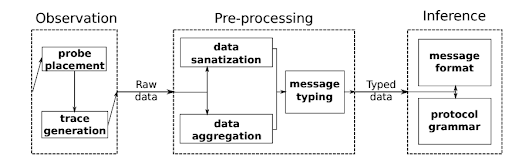
\includegraphics[width=\linewidth]{protocol_analysis_process.png}
    \label{fig:protocolanalysis}
\end{figure}
\section{Compiled Code RE}
It is important for a reverser to understand the different goals of high level and low level languages. 
Understanding these differences will help with interpretation of why code is structured a certain way.

\subsection{High level languages}
High level languages exist as an abstraction to interface with operating system software and underlying hardware.
High level languages work so a programmer can focus on specifying program implementation logic and structural design without needing to dedicate time to figuring out system specific details. If a programmer were to decide to write instructions to the machine they would use assembly language, a low-level, human readable language used to communicate more directly with the computer hardware. Those instructions would then get turned into machine code, an even lower level programming language that is readable to a computer's processor.
Compiled languages are very performant as they are converted to assembly language then machine code. Writing directly in assembly language could allow for optimizations, but compilers are pretty good at enacting those optimizations themselves. When interpreters or VMs (like the Java Virtual Machine) are involved, the VM invokes the necessary behaviors unlike in languages such as C or C++ where the compiled code becomes machine code for the target platform to run directly. 
While writing in something like assembly language can be very performant, it would be significantly more difficult and time consuming for a person to write a modern application in assembly.
High level languages remove the need for programmers to understand their program at the assembly level, a reverse engineer however is forced to examine the low-level assembly version of a compiled program to understand the specific ways a program's goals are being achieved.
The main goal of a reverse engineer is to use what they know about a program's behavior, the potential ways that can be accomplished in high level code, and how to read assembly code to determine specific instrumentation details.
For reverse engineers, the most important thing to know about a high level language is to what level does it abstract or conceal the underlying machine code~\cite{Reversing}. 

Languages like Python that have a built in interpreter will abstract it a lot. 
These programs may be full of extraneous instructions to perform necessary operations. On the other hand, languages like C are written much closer to the target processor and won’t have nearly as much separation between the source and machine code

\subsubsection{Control Flow}
Control flow is what makes code determine what instructions get executed and how often.
This manifests through statements like conditionals that give general instructions for what a program should do when a condition is true or false.
A processor has no knowledge what statements like ‘if’ or ‘while’ mean. 
Under the hood, these statements translate into verbose and daunting assembly code. 
This is because high level conditional statements are often broken down into a series of smaller operation sequences to match the instruction set the processor understnads~\cite{Reversing}.

Other typical structural components of programs that aid in control flow are switch blocks and loops. 
Switch blocks, or \(n-way\) conditionals, take in an input and have \(n\) number of code blocks that are potentially executed depending on the input value. 
Each block of code gets assigned at least one value prior to runtime. 
The compiler also generates code to receive the input value and search for the proper code block to execute. 
The values for the code blocks are usually stored in a lookup table that has pointers to each corresponding code block.  
Depending on the input value, the program will go through the process of searching the lookup table then jumping to the proper code block at runtime~\cite{Reversing}. 
Loops work to allow a program to repeatedly execute a certain code block multiple times. A loop has a counter to keep track of how many iterations it has performed. 
There is also a conditional statement that determines when the loop will stop. 
Loops and conditionals are inherently intertwined. 
The difference is that loops execute over and over until the condition is no longer met.

To understand control flow sequences, one must understand how low level control flow is implemented. 
This means that a reverse engineer needs to know the specific rules of each kind of low level architecture because low level control flow instructions are unique to the platform for which they are designed.

\subsection{Low level languages}
Earlier we mentioned that complexity is introduced when working with low level system specific details. 
This is especially true when the goal is to translate high level logic into something that will be understood by your machine. 
Of course, there must be a way to do this because the CPU does it anytime a modern application is run. 
But it often involves keeping track of more details than a sole human is capable of. 
That is why a reverse engineer must develop the skill of parsing through assembly code and being able to create a kind of ‘mental image’ of how it relates to high level constructs.
Data management is one of the things that a person’s computer keeps track of that would be difficult for a human to do.
To understand why this is, we can look at the data management of a relatively low level language, C, versus the assembly representation. 
Consider the code: 
\begin{figure}[H]
\centering
\begin{minipage}{0.33\textwidth}
\caption{Divide function code}
\begin{lstlisting}
int divide(int a, int b) {
    int result;
    result = a / b;
    return result;
}
\end{lstlisting}
\end{minipage}%
\hfill
\begin{minipage}{0.3\textwidth}
    \centering
    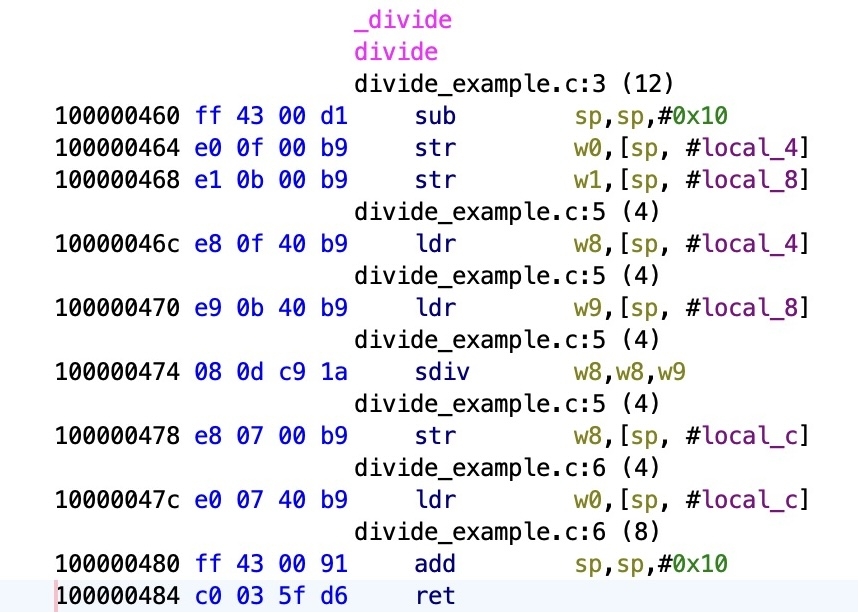
\includegraphics[width=\linewidth]{divide_ghidra.jpeg}
    \caption{Disassembly view in Ghidra}
    \label{fig:ghidra1}
\end{minipage}%
\hfill
\begin{minipage}{0.3\textwidth}
    \centering
    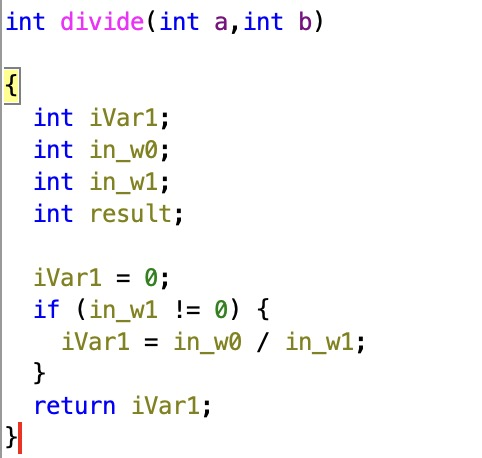
\includegraphics[width=\linewidth]{divide_ghidra2.jpeg}
    \caption{Decompiled code view in Ghidra}
    \label{fig:ghidra2}
\end{minipage}
\end{figure}

While this function may seem incredibly simple, there is no direct translation into a machine code representation. 
To execute this in a low level language, it would require first storing the machine state. 
Then memory would need to get allocated for result. Variables a and b would need to get loaded from memory into a register. 
Then a would need to be divided by b and the result would need to get stored in the register that got loaded in the beginning. 
The machine state from before would need to get reloaded. The pointer would need to return to the caller and bring back result~\cite{Reversing}.
One line of high level code could result in any number of assembly instructions.
Managing data is one of the biggest challenges of reverse engineering.


\subsubsection{Registers}
To keep from needing to constantly access RAM, microprocessors have a smaller internal memory that can be accessed with barely any performance cost~\cite{Reversing}. 
There are multiple types of internal memories that microprocessors keep and registers are one of them.
Registers are little pieces of internal memory that live within the processor and are able to be accessed with an imperceptible cost to performance~\cite{PracticalRE}. Data must be in a register in order for the CPU to access it for processing. 
The biggest problem with registers is that there are not very many of them. 
One of the most popular processors, the IA-32, only has eight 32-bit registers that can be used for anything. 
It does have more registers, but they all have highly specific use cases. 
Assembly language is written around utilizing registers because they’re so performant. 
They are not good for long term storage, though, that is when RAM becomes the better choice.

RAM is volatile memory, meaning its contents are lost when the computer is powered off. It temporarily holds data and instructions for currently active tasks, giving the CPU quick access to the broader context of running programs. The CPU operates using something called the instruction cycle: first, it fetches an instruction; then, it decodes or interprets it to determine the required operation; finally, it executes the instruction, carrying out the specified task.

One of the most important things to take away is that CPUs do not automatically manage these tasks. 
Data management is outlined in the assembly code which is what reverse engineers will need to get comfortable sorting through.
One thing that reverse engineers will need to do is focus on figuring out what kind of values are getting loaded into a register. 
For example, it is easy to see when a register is only being used to grant instructions access to a specific value because that register will only show up when transferring value from memory to the instruction or vice versa.
Another example is when a register shows up many times in one function. 
This is a good clue that one of the function's local variables is being stored in that register. Figure \ref{fig:registerdiagram} shows some of the different registers and their purposes.
\begin{figure}[H]
	\caption{Register and Flag descriptions and purposes}
	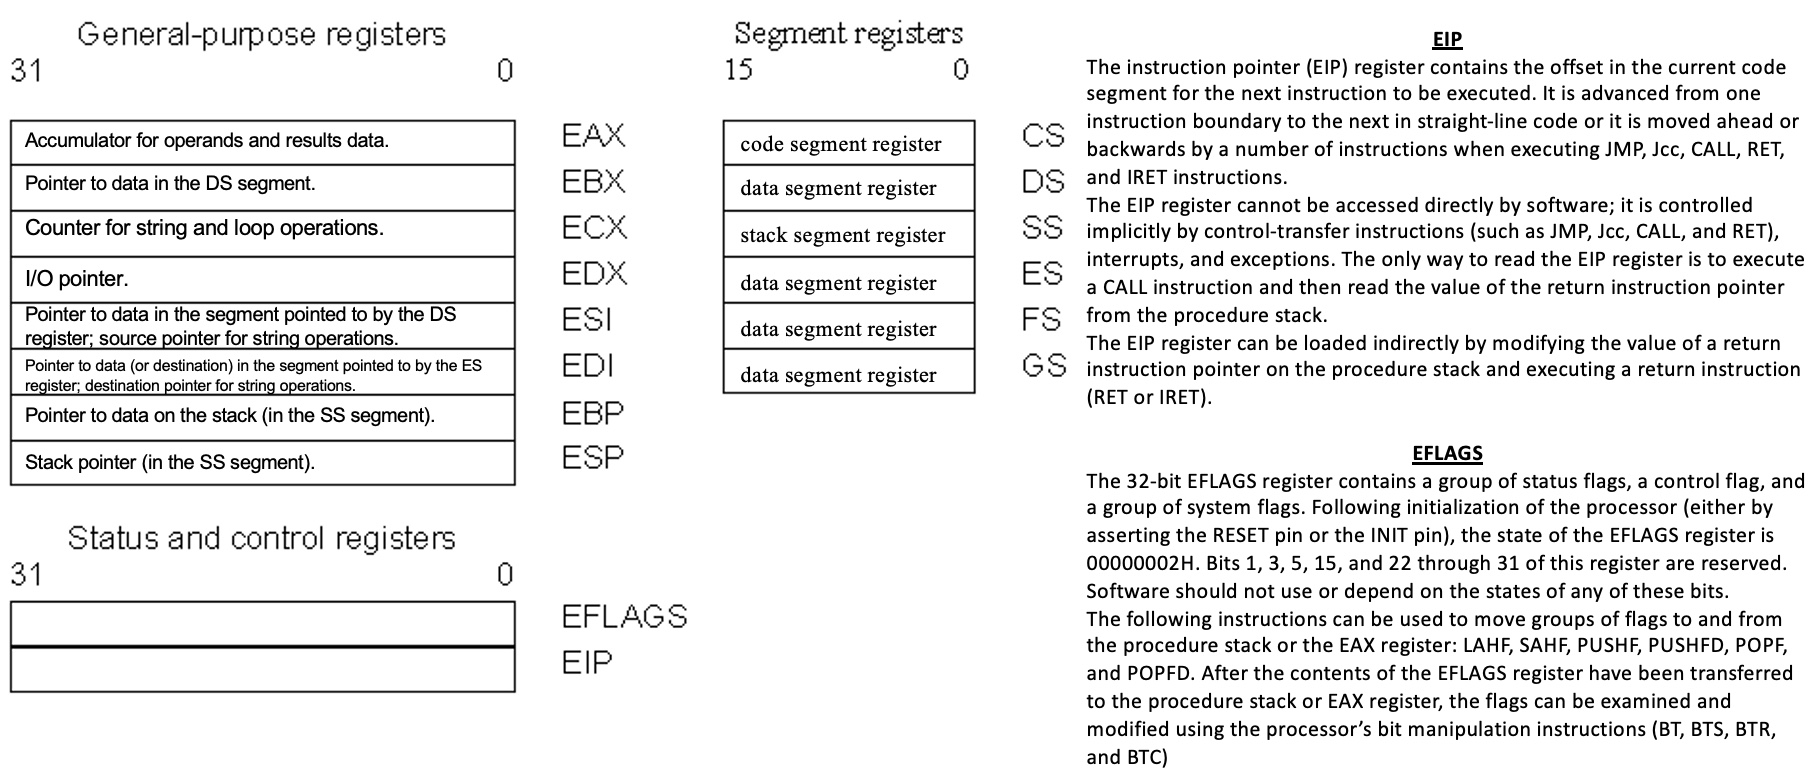
\includegraphics[scale=.27]{Register Diagram.jpeg}
    \label{fig:registerdiagram}
\end{figure}
\footnote{Figure modified using Intel® 64 and IA-32 Architectures Software Developer’s Manual and https://flint.cs.yale.edu/cs422/doc/pc-arch.html\#register}

\subsubsection{The Stack}
The stack is one of two places that a value can be set aside. 
Registers are not managed by a processor and to use one you just need to load a value in it. 
Often there will not be registers available or there is a particular reason a variable will need to reside in RAM instead of in a register. 
That’s when you’d put a variable on the stack instead~\cite{Reversing}.

The stack is a short term storage space in memory that gets utilized by both the CPU and the program. 
It is the spot where short term information gets put when a register can not be used for whatever reason. 
Registers are for the shortest term data while the stack is for the second shortest. 
The stack lives in RAM like all other data and is just a carved out section for intermediate term data. 
Modern operating systems tend to manage multiple stacks at the same time. 
Each of the concurrently running stacks is a representation of a program or thread~\cite{MasteringRE}.

Stacks use Last In First Out data management. 
Items are pushed on the top of the stack and popped from the top of the stack. 
Memory in stacks is allocated from the top down where the first in address is allocated and used first while the stack grows backwards towards lower addresses~\cite{Reversing}.

\subsubsection{Flags}
One of the registers you may have noticed from the previous figure \ref{fig:registerdiagram} is the EFLAGS register. 
This is a collection of special IA-32 registers that contain system and status flags. 
The system flags’ job is to manage the different modes and states of the processor. 
The status flags are what a reverse engineer will typically be more interested in and are used by the processor to record its current logical state~\cite{Reversing}. 
They are often updated by various logical and integer instructions so they can record the outcome of these actions. 
There are also instructions whose operation conditions are dependent on the values for the status flags. 
This is what allows sequences of instructions to run different operations depending on what different input values may be, etc. 

Flags in IA-32 are the crux of conditional code. 
Arithmetic instructions check operand conditions and then set processor flag conditions based on the resulting values. 
There are also sets of instructions designed to read the flags and do different operations based on the value. 
An example of a popular instruction set is Jcc or the Conditional Jump. 
It tests for predefined flag values and then jump depending on whether or not it matches with the specified conditional code~\cite{intelManual}.

\subsubsection{Functions}
Instructions are the actual actions specified in assembly code. 
They are formatted with operation code (opcode) and one or two operands~\cite{Reversing} 
The opcode is what you are asking the computer to do such as MOV or JMP. 
The operand is the parameters that get passed to the opcode or the data being manipulated. 
Certain instructions will have no parameters. Data in assembly comes in three basic forms. 
There are register names, immediate data, and memory addresses. 
Register names are the names of the general purpose registers to be read from or written to like the EAX, EBX, etc. 
Immediate data is constant values that are embedded into the code and usually indicates there was a hard coded value in the source code. 
Memory addresses are the locations of operands stored in RAM. 
It can be hard coded and tell the processor where to read to and write from. 
It could also be a register with a value that will be used as a memory address. 
It is also possible to combine a register with an arithmetic operation and a constant so that there is some base address and then an index offset~\cite{Reversing}.

General purpose instructions are the ones that deal with program flow, logic, arithmetic, string operations, and basic data movement. 
They deal with data stored in memory at the general purpose registers, EFLAGS register, segment registers, and address information stored in memory ~\cite{Reversing}.

The MOV instruction shows up most frequently in most IA-32 instruction sets. 
This one deals with basic data movement. 
It takes in a destination operand and a source operand then moves the data from the source to the destination. 
The sources can be registers, immediate, or memory addresses. 
It is important to note that MOV cannot transfer data through memory, it can only take it out or put it in. 
The destination address can be a memory address (using a register or an immediate) or a register~\cite{Reversing}.




\section{Example Problems}
With some grounding in reverse engineering tools, methods, and assembly, it's a good time to try out a few practice problems. There are a couple of ways to approach this. One option is to work on “CrackMe” challenges, which are small programs designed to test reverse engineering skills by making analysis deliberately difficult. Another approach is to reverse a self-written program, placing markers in the code to check whether they can be identified during analysis. 

\subsection{Reversing Hello World}
Before taking on the larger endeavor of reversing a program written in a declarative language (SwiftUI), it’s important to start with the basics. 
Figure \ref{fig:helloworldsource} shows a simple ‘Hello World’ program in C. 
To add some complexity, a few random variables and data structures were thrown in as Easter eggs. 
This is the program whose decompilation will be used as a jumping off point.
\begin{figure}[h]
	\caption{Hello World Program}
	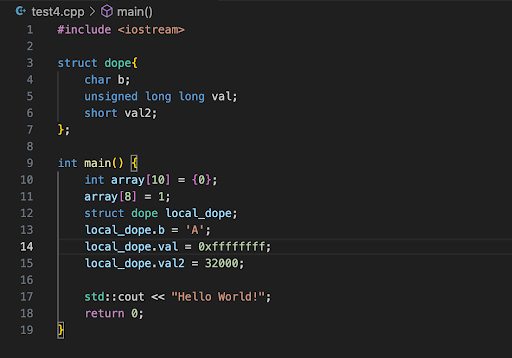
\includegraphics[scale=.75]{HelloWorldSource.png}
        \label{fig:helloworldsource}
\end{figure}
Figure \ref{fig:hellowworldghidra} is the decompilation of the program once it was put through Ghidra. 
The first thing to note is how with even a relatively low level language like C, the instructions in the code more than doubled. 
The disassembly being shown in the figure is also only a portion of Ghidra’s output. 
The figure only shows the function section of the program output when imports, exports, labels, classes, etc take up the large majority of the program. 
One important part of reverse engineering is sorting through all of the information to find out what exactly is important to the reverser. 
Some reverse engineers refer to this process as finding the shape and edges of the data. 
\begin{figure}[h]
	\caption{Hello World Disassembly}
	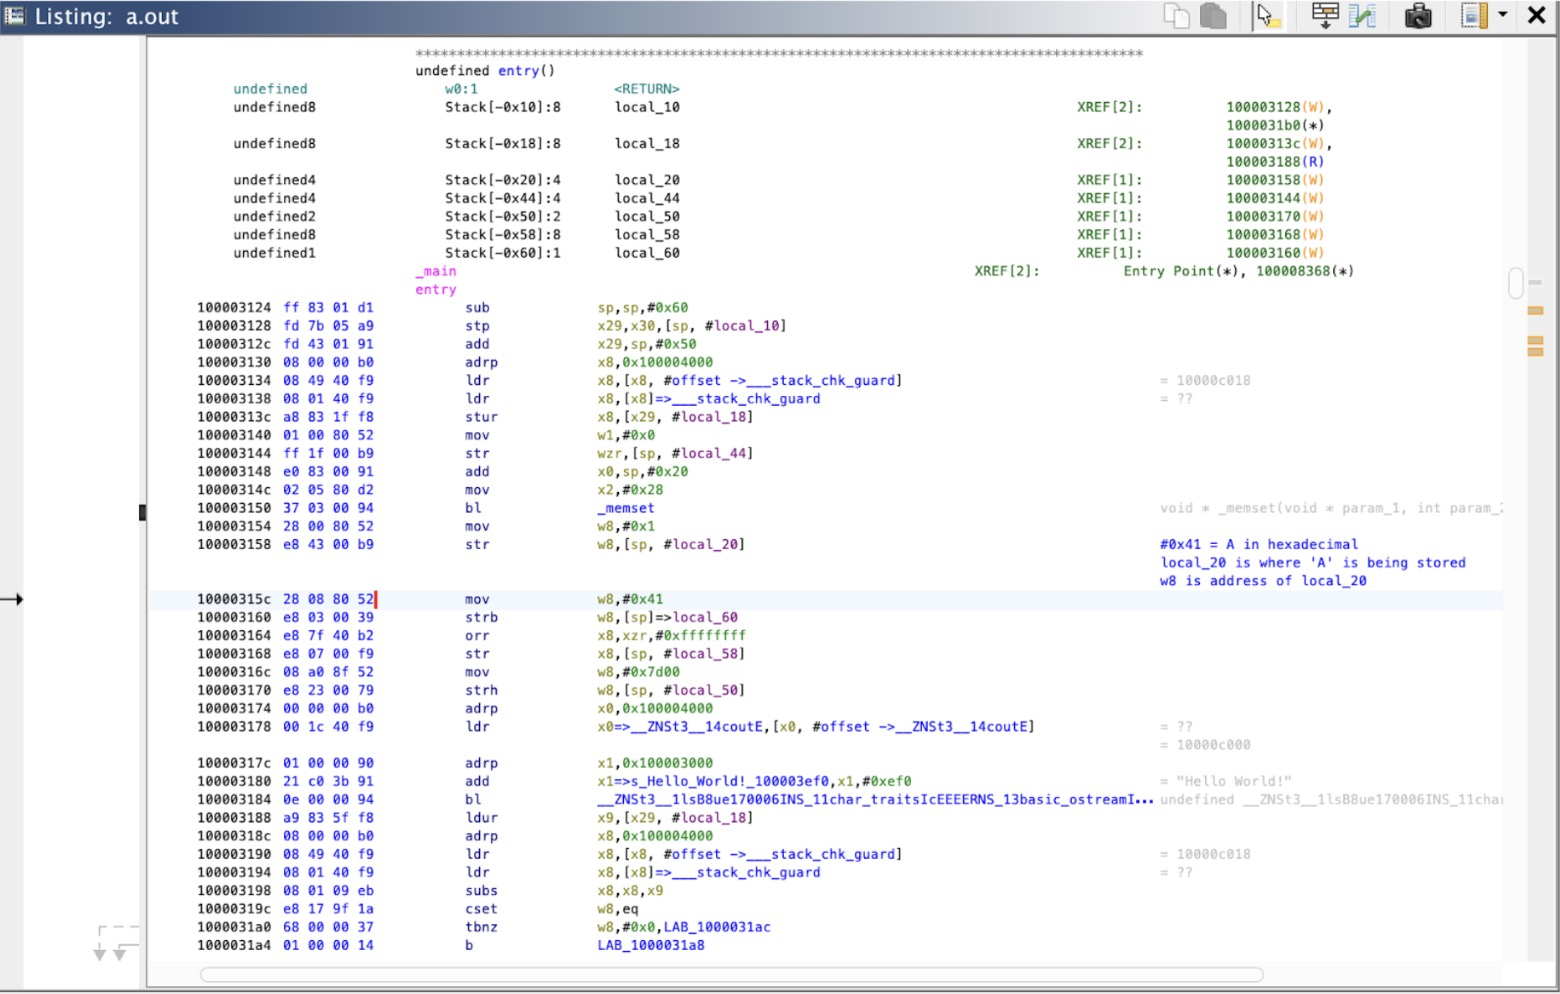
\includegraphics[scale=.3]{HelloWorldGhidra.png}
        \label{fig:hellowworldghidra}
\end{figure}
With the important section identified, it is time to analyze the assembly code.
One thing to keep in mind with the disassembled code is that all the values will be stored in hexadecimal. 
A good place to start is with the values we know will need to be stored. 
In the array there are 10 variables which all get set to 0, except for the eighth array member which is changed to equal 1. 
In our local\_dope struct there are three variables equal to ‘A’, ‘0xffffffff’, and 32000. 
The highlighted line in the figure shows ‘A’ being stored in the register w8. Shortly after, \#0xfffffff shows up without needing to be translated into hexadecimal. 
\#0x7d000 is the hex for 32000. 
This surface level analysis offers a glimpse into the methodology of more complex reverse engineering. 
Lastly, the 'Hello\_World!' gives us the final piece of information we need to know about what the program is.

\subsection{Crack Me}
The next step in practicing reverse engineering is trying a Crack Me problem. 
Crack Me problems are toy problems designed by other software developers to help reverser's practice their skills. 
Usually there’s an executable that opens up a little puzzle. 
The puzzles usually involve finding a password but can involve any number of things like decryption, key generation, etc. 
This section will cover the process of reverse engineering a simple crack me.

The first step I took in reversing this program was checking the header and libraries as shown in Figure \ref{fig:crackmeheader} and \ref{fig:crackmelibs}.
\begin{figure}[H]
	\caption{Crack Me Header}
	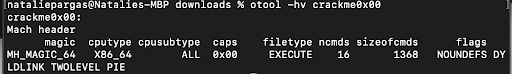
\includegraphics[width=\linewidth] {crackmeheader.png}
        \label{fig:crackmeheader}
\end{figure}
\begin{figure}[H]
    \centering
    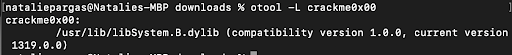
\includegraphics[width=\linewidth]{crackmelibs.png}
    \caption{Crack Me Libraries}
    \label{fig:crackmelibs}
\end{figure}



Both of these steps were done with an executable dumping tool called ‘otool’. 
The header information shows that the assembly language being used is x86. 
The library dump shows that the only library being linked is the system library. 
While these tools didn’t offer that much information about this particular program, they are very useful in programs that have more dependencies and more specific assembly languages. 
These dumping tools ended up being vital later in the project because they offered insight into what libraries were being linked from the project's declarative language as well as what assembly language was being used with Apple’s modified version of ARM64. 
Next, otool was used once again to list the strings. 
This is a vital part of reverse engineering and is useful to be able to refer back to during the process. 
Figure \ref{fig:crackmestrings} shows the result of the string dump.


\begin{figure}[H]
	\caption{Crack Me Strings}
	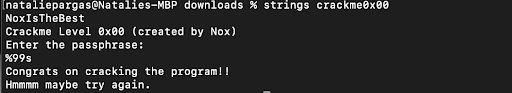
\includegraphics[width=\linewidth]{crackmestrings.png}
        \label{fig:crackmestrings}
\end{figure}

Examining this more closely, you can see that there’s only a few strings that give a very clear idea of what the program is designed to do. 
There’s a random string, the title of the program, a passphrase prompt, a string indicating the expected input, a congratulations message, and an incorrect guess message. 
With just this information, you could easily make an educated guess on what the password is. 
Most likely the passphrase will be the one random string that doesn’t get given easily in the executable. 
But for the sake of gaining understanding of the process, it’s good to go over the decompiled code. 
Figure \ref{fig:crackmeghidra} shows the decompiled code.
\begin{figure}[H]
	\caption{Crack Me Ghidra Disassembly}
	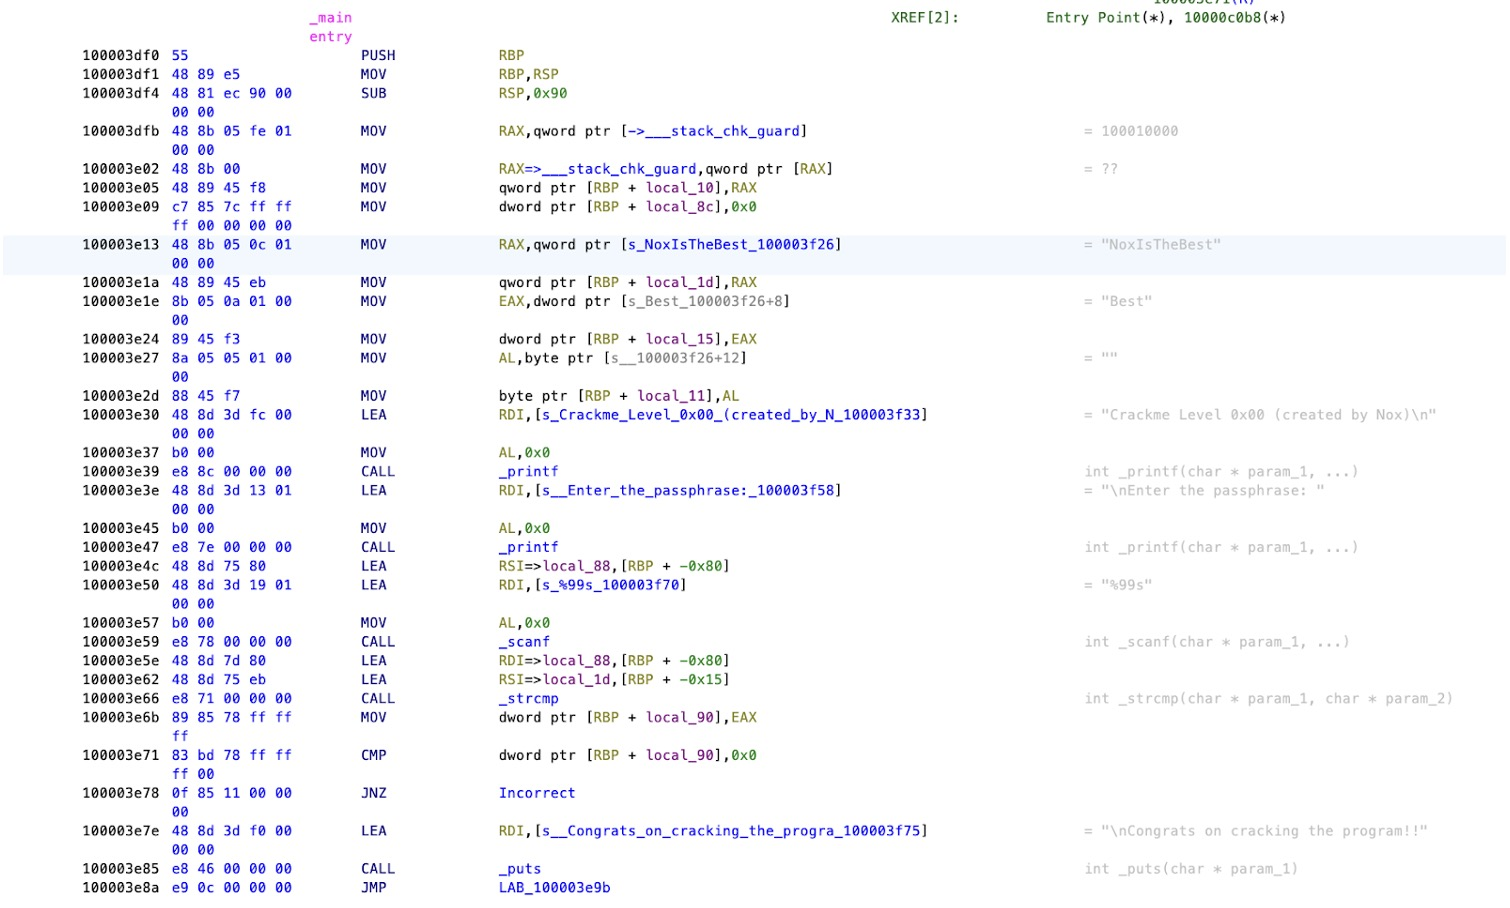
\includegraphics[scale=.25]{crackmeghidra.png}
        \label{fig:crackmeghidra}
\end{figure}

The first thing to do is find the entrance into the program. 
Ghidra already labeled the ‘\_main’ at the top but the strings and function calls reaffirm this as the right section to be looking over. 
Next, thinking back to the string dump, it’s likely that the password will be near whatever function takes input. 
Prior knowledge of programming informs the reverser that after getting the user input, the input string will need to be compared to the right answer. 
Thankfully Ghidra was able to identify the function ‘scanf’.

\begin{figure}[H]
	\caption{Crack Me Code Section 1}
	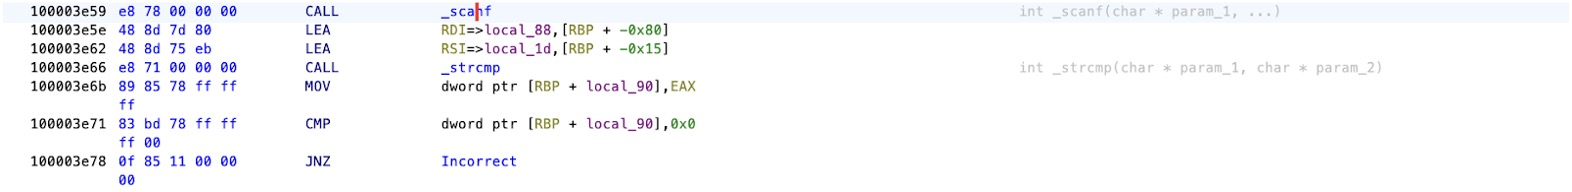
\includegraphics[scale=.3]{crackmescanf.png}
        \label{fig:crackme1}
\end{figure}

Inspecting the code section at Figure \ref{fig:crackme1}, it shows that the variable local\_88 contains the user input. 
This is because it loads a \%99s into the RDI register to prepare for the input directly above where scanf is called. 
RSI has local\_1d loaded into it and that variable is immediately ‘strcmp’ compared to local\_88. Using these clues, one could infer that local\_1d contains the password. 
To verify, a reverser should always retrace and check.

\begin{figure}[H]
	\caption{Crack Me Code Section 2}
	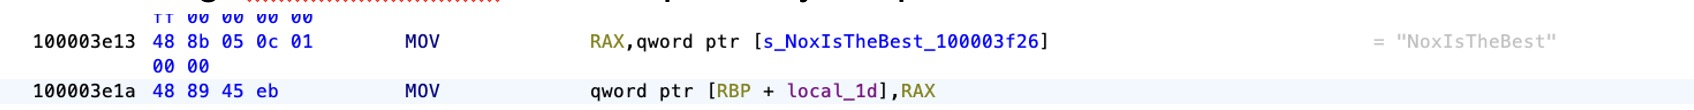
\includegraphics[scale=.3]{crackmeRAX.png}
\end{figure}

The first instance of local\_1d contains the register RAX 9. 
RAX has the qword ptr ‘ s\_NoxIsTheBest\_100003f26’ moved into it right above. 
s\_NoxIsTheBest\_100003f25 only contains the string “NoxIsTheBest”. 
That string is probably the password, but all that’s left is to check. 
Figure \ref{fig:crackmeexe} shows the result.
\begin{figure}[H]
	\caption{Crack Me Code Executable}
	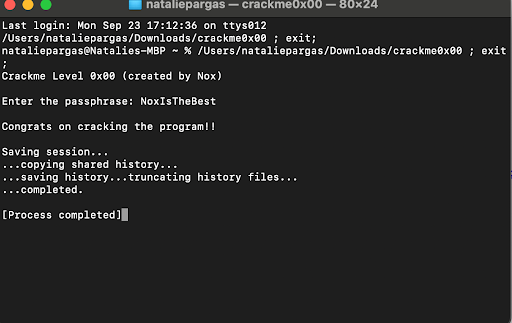
\includegraphics[scale=.6]{crackmeexe.png}
        \label{fig:crackmeexe}
\end{figure}
The attempt was a success and the crack me was successfully reverse engineered!

